% \pagecolor{red!10}
\section*{Level 0 (Children)}
\noindent
\resizebox{1\textwidth}{!}{
    %%%%%%%%%%%%%%%%%%%%%%%%%%%%%%%%%%%%%%%%%%%%%%%%%%%%
    %%% SHAOBAN
    %%%%%%%%%%%%%%%%%%%%%%%%%%%%%%%%%%%%%%%%%%%%%%%%%%%%
	\begin{tikzpicture}[font=\footnotesize,node distance=0em]
		% Frame
		\fill[yellow!10, draw=black, rounded corners] ($(0,0) + (-0.25cm,0.25cm)$) rectangle (8cm,-12cm);	
	
		\node[below right] at (8cm-2cm-0.25cm-0.25cm,0) {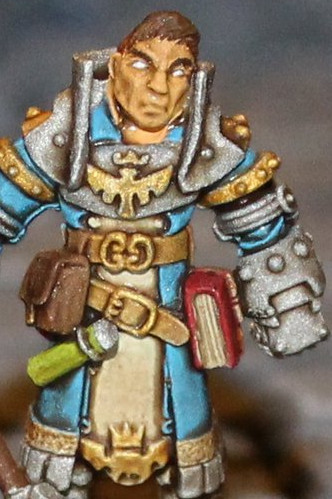
\includegraphics[width=2cm, height=3cm]{C:/privat/rpg/crimson_throne_book/latex/images/shaoban}};
	
		\node[below right,font=\bfseries\setmainfont{Immortal}\large] (name) at (0,0) {SHAOBAN};

		\node[below=of name.south west,below right,yshift=0.5em] (info){LN small human};
		
		\node[below=of info.south west,below right, align=left] (skills) {
                Init +0; Senses Perception +2\\ 
                Common
		};

		\node[below=of skills.south west,below right, align=left] (ac){
                AC 11, touch 11, flat-footed 11\\
                HP 5 (1HD)\\
                Fort -1, Ref +0, Will +2
		};
	

		\node[below=of ac.south west,below right, align=left] (fight) {
                Speed 30 ft. (6 squares)\\
                Melee dagger (small) +1 (1d3/19-20)\\
                Ranged dagger (small/thrown) +1 (1d3/19-20)\\
                Face 5 ft. Reach 5 ft.\\
                Base Atk +0; CMB -1; CMD 9
        };

		\node[below=of fight.south west,below right, align=left] (abilities) {
                Str 10, Dex 10, Con 8, Int 8, Wis 14, Cha 18
	   };

		\node[below=of abilities.south west,below right, align=left] (feats) {
                Simple Weapon Proficiency
	   };

		\node[below=of feats.south west,below right, align=left, text width=7.5cm] (skills) {
            Appraise -1, Bluff +4, Diplomacy +7, Disguise +4,\\ 
            Fly +2, Heal +2, Intimidate +5, Perception +2,\\ 
            Sense Motive +6, Sleight of Hand +6, Stealth +4,\\ 
            Survival +2
	   };

		\node[below=of skills.south west,below right, align=left, text width=7.5cm] (poss) {
            Dagger (small) 
	   };
	
		\node[below=of poss.south west,below right, align=left, text width=7.5cm] (traits) {
            {\itshape Child of the Streets:} {\scriptsize You grew up on the streets of a large city, and as a result you have developed a knack for picking pockets and hiding small objects on your person. You gain a +1 trait bonus on Sleight of Hand checks, and Sleight of Hand is always a class skill for you.}\\
            {\itshape Ease of Faith:} {\scriptsize  Your mentor, the person who invested your faith in you from an early age, took steps to ensure that you understood that what powers your divine magic is no different than that which powers the magic of other religions. You gain a +1 trait bonus on Diplomacy checks, and Diplomacy is always a class skill for you.}
        };
	\end{tikzpicture}
    \hspace{0.25cm}
    %%%%%%%%%%%%%%%%%%%%%%%%%%%%%%%%%%%%%%%%%%%%%%%%%%%%
    %%% Quintilian
    %%%%%%%%%%%%%%%%%%%%%%%%%%%%%%%%%%%%%%%%%%%%%%%%%%%%
	\begin{tikzpicture}[font=\footnotesize,node distance=0em]
		% Frame
		\fill[yellow!10, draw=black, rounded corners] ($(0,0) + (-0.25cm,0.25cm)$) rectangle (8cm,-12cm); 
    
        \node[below right] at (8cm-2cm-0.25cm-0.25cm,0) {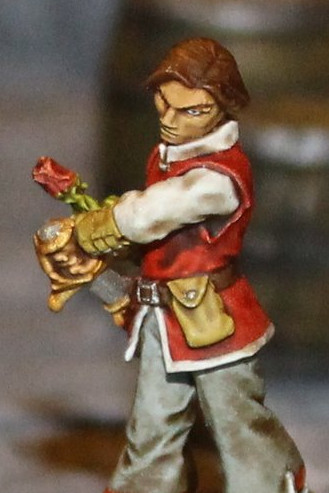
\includegraphics[width=2cm, height=3cm]{C:/privat/rpg/crimson_throne_book/latex/images/quint}};
    
        \node[below right,font=\bfseries\setmainfont{Immortal}\large] (name) at (0,0) {QUINTILIAN};

        \node[below=of name.south west,below right,yshift=0.5em] (info){CG small human};
        
        \node[below=of info.south west,below right, align=left] (skills) {
                Init +2; Senses Perception -1\\ 
                Common
        };

        \node[below=of skills.south west,below right, align=left] (ac){
                AC 13, touch 13, flat-footed 11\\
                HP 5 (1HD)\\
                Fort -1, Ref +2, Will -1
        };
    

        \node[below=of ac.south west,below right, align=left] (fight) {
                Speed 30 ft. (6 squares)\\
                Melee dagger (small) +1 (1d3/19-20)\\
                Ranged dagger (small/thrown) +1 (1d3/19-20)\\
                Face 5 ft. Reach 5 ft.\\
                Base Atk +0; CMB -1; CMD 11
        };

        \node[below=of fight.south west,below right, align=left] (abilities) {
                Str 10, Dex 14, Con 8, Int 14, Wis 8, Cha 16
       };
	\end{tikzpicture}
}

\vfill
\noindent
\resizebox{1\textwidth}{!}{
	\begin{tikzpicture}
		% Frame
		\fill[yellow!10, draw=black, rounded corners] ($(0,0) + (-0.25cm,0.25cm)$) rectangle (8cm,-12cm);	
	
		\node[below right] at (8cm-3cm-0.25cm-0.25cm,0) {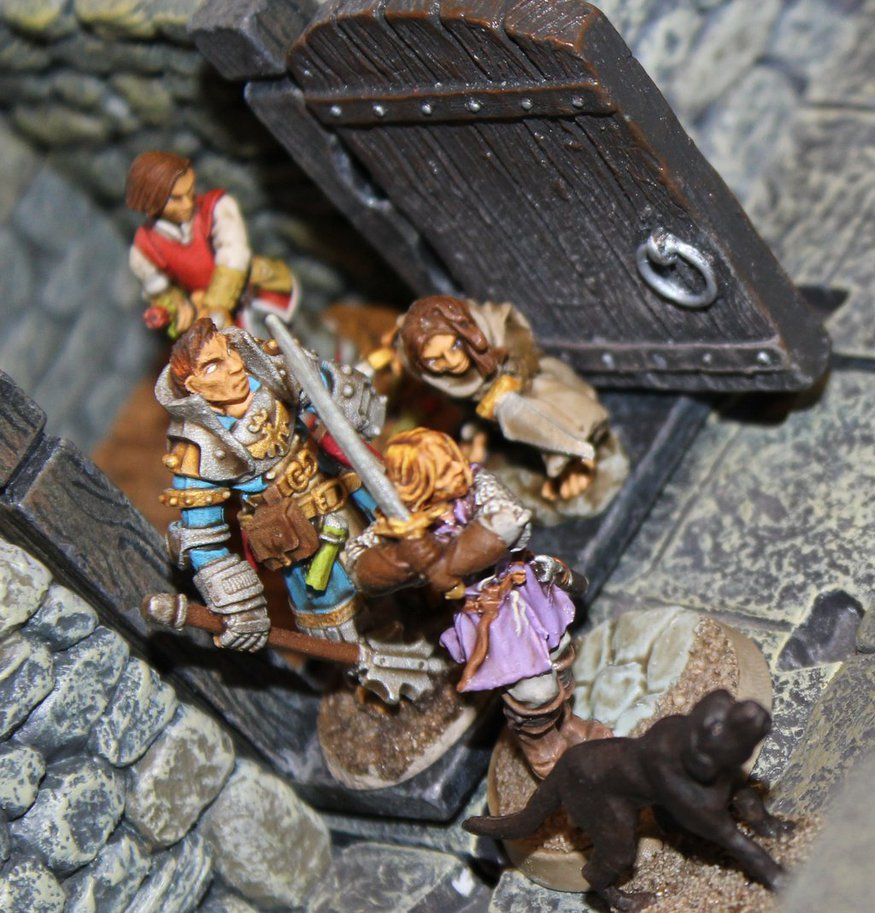
\includegraphics[width=3cm, height=4cm]{C:/privat/rpg/crimson_throne_book/latex/images/titlepage}};
	
		\node[below right,font=\bfseries\setmainfont{Immortal}\large] (name) at (0,0) {BALIAN};
		\node[below right] at (0, -0.45cm) {LN small human};
	
	% Init +0; Senses Perception +2
	% Languages Common
	% AC 11, touch 11, flat-footed 11
	% hp 5 (1HD)
	% Fort -1, Ref +0, Will +2
	% Speed 30 ft. (6 squares)
	% Melee dagger (small) +1 (1d3/19-20)
	% Ranged dagger (small/thrown) +1 (1d3/19-20)
	% Face 5 ft. Reach 5 ft.
	% Base Atk +0; CMB -1; CMD 9
	% Abilities Str 10, Dex 10, Con 8, Int 8, Wis 14, Cha 18
	
	
	
	\end{tikzpicture}
\hspace{0.25cm}
	\begin{tikzpicture}
		% Frame
		\fill[white, draw=none, rounded corners] ($(0,0) + (-0.25cm,0.25cm)$) rectangle (8cm,-12cm);	
	
		% \node[below right] at (8cm-3cm-0.25cm-0.25cm,0) {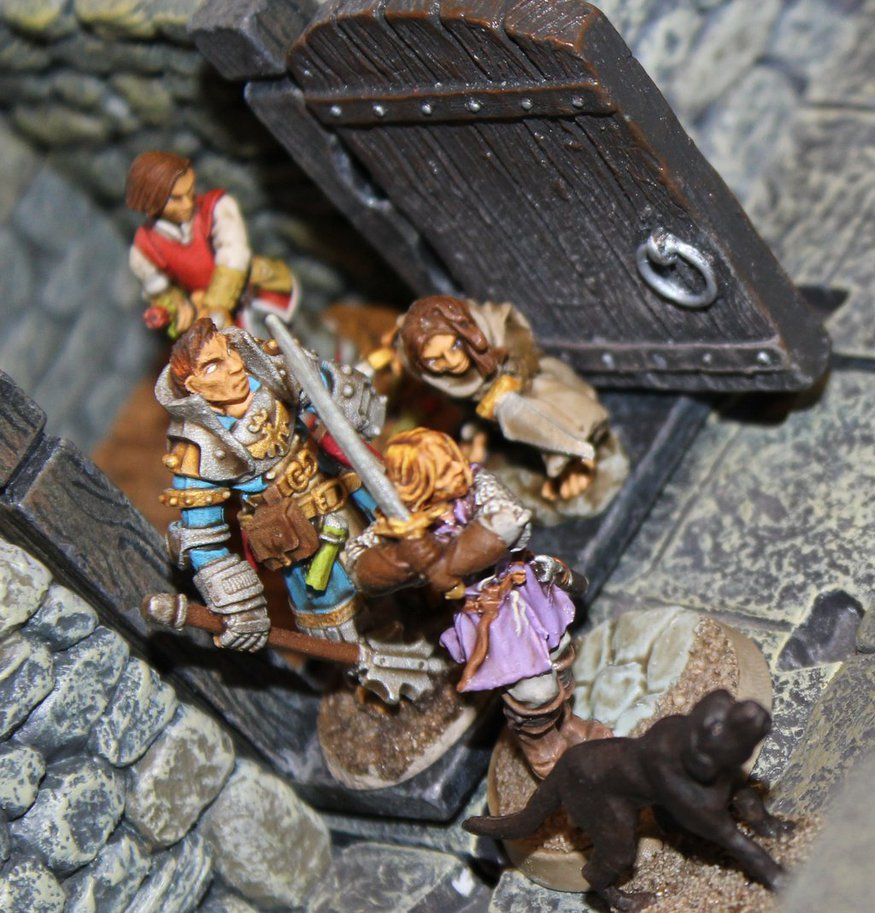
\includegraphics[width=3cm, height=4cm]{C:/privat/rpg/crimson_throne_book/latex/images/titlepage}};
	
		% \node[below right,font=\bfseries\setmainfont{Immortal}\large] (name) at (0,0) {PUK};
		% \node[below right] at (0, -0.45cm) {LN small human};
	
	% Init +0; Senses Perception +2
	% Languages Common
	% AC 11, touch 11, flat-footed 11
	% hp 5 (1HD)
	% Fort -1, Ref +0, Will +2
	% Speed 30 ft. (6 squares)
	% Melee dagger (small) +1 (1d3/19-20)
	% Ranged dagger (small/thrown) +1 (1d3/19-20)
	% Face 5 ft. Reach 5 ft.
	% Base Atk +0; CMB -1; CMD 9
	% Abilities Str 10, Dex 10, Con 8, Int 8, Wis 14, Cha 18
	
	
	
	\end{tikzpicture}
}